
% !TeX spellcheck = en_US


\chapter{Introduction}
\section{Problem Statement and Benefits}%
 
 \marginpar{Motivation\\ \cite{techopedia2022}, \cite{Choudhry2018}, \cite{Parsick2018}}%
 In the last 20 years, agile approaches have spread in their popularity. One principle of agile methods is how to deal with change. This has changed massively compared to previous, not agile methods. For example, in agile development, changes are allowed even in the late stages of the project. However, the database community has traditionally considered database design to be something that is planned.
 
Keeping track of database changes in complex and agile company environments is tough. Handling relational database changes requires special consideration and offers different challenges than deploying classical software. Database systems need help with problems such as untracked changes, overwritten code, data loss or mix-ups. Such shortcomings applied to the production database can be a significant risk. Manual modification of database structures can be very time-consuming and error-prone. Nobody knows which database scripts are applied to which database instances. 
Without a clearly defined process, database migration scripts are recorded, for example, on release notes or ticket systems.
In addition, no one may know how the test database differs from the production database.
 
For that reason, migrations are best done automatically to avoid downtime or errors. In addition, proper database change management ensures that changes to a database are controlled and safe. According to \cite{ManageForce2016}, 80\% of unplanned database downtime is due to database changes.
Developers need an excellent strategy for how to apply changes to the same database environment.
This problem requires a best practices strategy for dealing with different users, branches and applications. It can quickly happen that when a change in the code results in a change in the database, the migration of the database is subsequently forgotten. Using a proper management system can prevent a developer from running into such errors where a database migration has been forgotten for example a very annoying \textit{Column not found} error.

\marginpar{SQL DDL/DML\ \cite{Fritchey2011}}%
However, why not just use SQL \gls{DDL}/\gls{DML} as a source for change management? SQL DDL and DML statements are used to create, modify, and query the structure and data of a database, respectively. While these statements can be used to make changes to a database, they are not suited for change management in the broader sense.

Change management refers to tracking, reviewing, approving, and implementing changes to a system or process. In the context of a database, this would involve not only making changes to the structure and data of the database using SQL statements but also documenting and communicating those changes to stakeholders, testing the changes to ensure that they have the desired effect and do not break any existing functionality, and rolling back changes if necessary.

Database change management systems are designed to support this process by providing a framework for managing and automating the entire change management process. These systems typically include features such as version control, change tracking, approval workflows, and rollback capabilities, which make it easier to manage and coordinate changes to a database.

Using a database change management system can help ensure that changes to a database are made controlled and consistently, reducing the risk of errors and downtime. It can also improve collaboration and communication among team members and make it easier to audit and document changes to the database.
 
\marginpar{Benefits}%
With the problems and shortcomings mentioned above, it is beneficial to implement certain automatism or use so-called change management tools in the deployment pipeline.
\cite{Dillon2022}, \cite{Robles2021}, and \cite{Fritchey2022} present the benefits a change management tool should provide or at least make it easier to use. The following list summarises the benefits of using database change management tools.

\begin{enumerate}
	\item Unique identification of all migrations and recording in a migration history table.
    \item Automatically deploy scripts and keep track whether they are already applied or not.
    \item Branching and merging for development in teams
    \item Embed easily into products or build tools.
    \item Make it easy to undo or revert changes without requiring a restore.
    \item Reproduce schema changes across multiple environments and auditing of these changes.
    \item Provide automation so you can do schema changes automatically without manual effort.
    \item An additional backup of the code that defines the database.
\end{enumerate}


Furthermore, migration can be used as the single source of truth for the actual production schemas. This becomes very handy once multiple database environments are updated with different deployment states.

\marginpar{Context}%
This seminar thesis focuses on database migrations in the context of schema migrations.  Other database migrations, such as moving a database to a different platform or a cloud, are not considered in the context of this work.

\newpage
\section{State of the Art}%
\subsection{DevOps strategies}
\marginpar{Change\\ management strategies\\ \cite{GoogleDevOps2022}, \cite{Piairo2018}}%
In most organizations, the way in which database changes are handled is different. There are the following common scenarios:

\begin{enumerate}
	\item \textit{Database changes are not included in the deployment pipeline}\\
	If changes in the database are not included in the pipeline, most migrations are performed manually, which results in risks and costs. Furthermore, not including the database changes leads to a lack of traceability and promotes the fear of every change.	
	
	\item \textit{Database and application changes have a different deployment process}\\
	Software developers use continuous delivery to manage their deployment of the software. The demand for techniques that support these agile processes is desired in a modern agile environment. Many teams use similar techniques regarding database change management and add their database changes as scripts in version control tools in a separate pipeline. Most developers know how to use software development tools very well and can apply these version control techniques to their database environment. However, if a database has an encapsulated pipeline to the application, the application development team and the administrator must keep it synchronized. As a result, agile delivery processes become slowed down by database deployment and synchronization with the application.

	Team members, including \gls{DBA}, need to see how changes are progressing to know what changes are planned, how their testing is going, and which schema changes have been implemented in production databases.
	
	\item \textit{Database and application share a deployment process}
	According to  \cite{GoogleDevOps2022}, this is the best pratice method which can be achieved by this:
	\begin{itemize}
		\item Keeping all database schema changes in version control, together with the application code the schema belongs to
		\item Using a tool that records which changes have been run against which environments, and what the results were.
	\end{itemize}
	These practices also ensure that there is a canonical source of truth for all changes and make the change history easily accessible for auditing purposes.

\end{enumerate}

\subsection{Deployment Workflows}
\marginpar{Multiple Environments \cite{Lukonin2017}}%
In many cases, three instances of the database are needed in parallel. One database for development is located locally with each developer. The second database is for testing purposes before deploying, and the third is the production database. Therefore, each developer should use his/her local database copy and branch.

Migration tools like Flyway or Liquibase can be used in these three environments. They allow local integration and use and integration into the CI pipeline in which the test database is used. Change management tools can also be integrated into the production environment, for example, in the cloud. The user can test the migrations directly locally. When it comes to deployment, a test can be performed automatically, for example on the test database. If this test is successful, the changes are only applied to the production database.

\subsection{Best Practices for database migrations \label{best_practices}}%
\marginpar{Best practices methods  \cite{Parsick2018}, \cite{F5works2017}, \cite{Langan2022}, \cite{Heppell2021}, \cite{Lukonin2017}}%
Specific best practices simplify dealing with database changes regardless of what strategy or tools a developer needs.

\begin{itemize}
	\item Use a version control system\\
	Whether a migration tool is used or not, it is advised to version control all artefacts like DDL, DML, test data, configurations, and functions with a \gls{VCS}.
	\item Automate the deployment process\\
	Manual changes can easily lead to mistakes and need manual rollbacks. Therefore use an automation and migration tool that can avoid costly mistakes and have the ability to roll back.
	\item Atomic changes\\
	For example, when a code change requires changing two database tables and patching existing data, there should be at least three scripts.
	\item Naming convention\\
	A team or company should agree on a naming convention for the migration files. It is recommended to use an ascending naming convention, for example, with increasing file names.
	
	\begin{lstlisting}[caption=Increasing file names]
		V001__first_change.sql
		V002__second_change.sql
		V003__third_change.sql
	\end{lstlisting}
	Instead of using integers to identify versions of the delta file, timestamps can significantly reduce the likelihood of conflicts. In addition, with timestamps, migrations can be applied in the order in which they were created, which helps to maintain the integrity of the database. 

	\begin{lstlisting}[caption=Timestamps]
		V2022-12-25-14-52__first_change.sql
		V2022-12-26-09-02__second_change.sql
		V2022-12-28-16-32__third_change.sql
	\end{lstlisting}

	This convention improves the handling of branches because, with this naming, the scripts are automatically sorted by date. However, if a branch containing an older migration script is merged into the main branch before a branch containing a newer script, for example, Flyway will ignore the older script by default. Flyway will consider the migration script in purple Branch \#2 to be outdated when merged. This is true regardless of whether the version numbers are timestamps or integers. To prevent this issue, enable the out-of-order migrations setting in Flyway, allowing it to apply migration scripts in any order.  
	
	\begin{figure}[H]
		\centering
		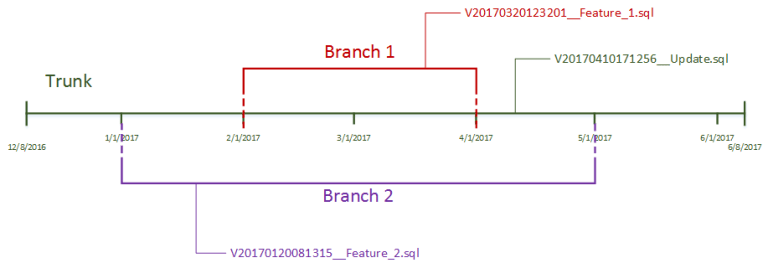
\includegraphics[width=0.95\textwidth]{./chapters/introduction/images/Branching-Flyway-Branch.png}
		\caption[Branching with Flyway - Source: \cite{Lukonin2017}]{Branching with Flyway}
		\label{fig:flyway_branching}
	\end{figure}
	
	\item Make sure to track all database changes\\
	Everyone should be able to see the latest change and history.
	\item Store current schema version number in database\\
	To check weather the most recent version is deployed.
	\item Test changes\\
	If two migrations share the same name or you make a change that is influenced by another developer, it can quickly lead to a crash of the migration. So every migration or change on database artifacts has to be tested before and after every merge to the main branch to catch issues straight away.
	\item Each developer uses his own database and test databases resemble the production database.
\end{itemize}


\newpage
\section{Available Tools}%
This section gives a non holistic excerpt about possible database change tools.
%The list of tools should include the available programming languages, price / availability
%and the main advantage over their competitors.

\begin{table}[H]
	\centering
	\ra{1.3}
	\begin{tabularx}{10cm}{X l l}
		\toprule
		Name & Language \\ 
		\midrule
		Flyway & independent \\
		Liquibase & independent \\
		migrate & Go  \\
		Active Record Migrations & Ruby on Rails \\
		alembic & Python \\
		dbup & .NET \\
		Visual Studio - SQL Server Data Tools & \\
		Entity Framework Migrations & .NET \\
		Laravel Migrations & PHP \\
		dbForge Source Control & \\
		Yoyo &  Python\\
		Phinx & PHP\\
		Source Control for Oracle & \\
		DBmaestro &  \\
		Django & Python \\
		DBdeploy & PHP \\
		FluentMigrator & .Net, C\#\\
		DBGeni & \\
		DB Ghost Change Manager & \\
		Version SQL & \\
		Sqitch & \\
		Idera DB Change Manager & \\
	\bottomrule
	\end{tabularx}
	\caption{Available migration tools - Based on \cite{GoogleCloudTools, DBMSTools}}
	\label{tab:migration_tools}
\end{table}

There are tools for different programming languages and in different qualities. These range from shell script-like repositories to enterprise solutions. In this work, however, only the two tools Flyway and Liquibase are examined and tested.




\section{Overview}%
This section will provide an overview of thesis.

